\chapter*{17.08. --- Pożegnanie z Islandią}

Jeszcze nigdy nie było nam tak ciężko się zebrać, jak w dniu dzisiejszym. Dolegujemy, przewracamy się z boku na bok, wymyślamy wymów\-ki dlaczego nie chcemy wypełznąć z namiotów. Wszystko to z bardzo prostego powodu --- mentalnie wyjazd skończył się wczoraj, z chwilą wjechania na \road{1} przed Reykjavikiem. Skończyło się obcowanie z naturą i ,,przygoda'', biwak na kempingu gdzie oprócz nas obozuje z pół tysiąca osób nie ma klimatu, otoczenie również nie nastraja optymistycznie. Zresztą --- znów do przejechania mamy zaledwie 50~km, więc \emph{,,po co się spieszyć? co będziemy robić w Asbru?!''}

Wczesne popołudnie upływa leniwie, na długich zakupach pamiątek w sklepach przy ulicy Laugavegur (to coś jak reykjawickie Krupówki). W sumie to dziewczyny kupowały, a ja z Putem siedzieliśmy na murku przed sklepem i ,,kontemplowaliśmy'' życie miejskie. Ktoś, kto by nas obserwował, mógłby z całą pewnością stwierdzić: ci dwaj goście mają \href{http://en.wikipedia.org/wiki/Thousand-yard_stare}{,,spojrzenie na 1000 jardów''} --- tym objawia się nagły kontakt ze zbyt dużą ilością bodźców i ludzi.

\img{./photos/x-s-2014-08-17_16-12-32__421.jpg}{is_this_the_end}{A więc\textellipsis to już koniec?!}

Tak sobie siedzimy na murku, gdy nagle zauważamy trzech starszych panów kręcących się koło nas i co chwila rzucających nerwowe spojrzenia w naszą stronę --- widać naradzają się, ale co takiego knują? Wreszcie jeden z nich podchodzi i pyta: \newline
--- \emph{Where are you from? I don’t see any country for this flag!} \newline
--- \emph{From Poland!} --- odpowiadamy. \newline
Na to jeden z nich stwierdza: \newline
--- \emph{Ale to powinna być flaga niebiesko-biało-czerwona, prawda?} \newline
Jego kompan protestuje --- kolory powinny znajdować się w odwrotnej kolejności! (Pewnie zrozumieli, jak to często bywa, ,,Holland'' zamiast ,,Poland''. \newline
--- \emph{To gdzie teraz?} --- zagajają dalej. \newline
--- \emph{Do domu, do Berlina, do Wa-wy\textellipsis} \newline
--- \emph{Aha, a ile kilometrów przejechaliście?} \newline
--- \emph{Dwa tysiące.} \newline
--- \emph{Z Warszawy?!} \newline
Ogólnie to straszne tępaki, aż zachodziliśmy w głowę gdzie takie się rodzą, lecz na do widzenia sami się przyznali: \emph{,,Greetings from Canada!''}

Po zakupach w butikach zajrzeliśmy na moment do katedry, potem na drugie śniadanie do Bonusa i\textellipsis znów ruszamy w trasę.

W połowie drogi do Ásbrú rozegrał się istny dramat. Zatrzymaliśmy się na postój, oparłem rower o stojącą na poboczu latarnię, a tu nagle --- jak nie huknęło! Ewidentnie coś eksplodowało i to eksplodowało w moim rowerze! Podejrzanych nie było wielu --- to znów feralna dętka w przednim kole. Najwyraźniej niemiecka łatka przetarła się (w końcu przejechała już blisko 200~km!) i zalegający pobocze ostry żwirek przeciął dętkę. Mniejsza o przyczyny, najgorsze że tego nie ma jak normalnie załatać! Zrezygnowany zaczynam iść dalej pieszo, lecz szybko przekonałem się, że to bez sensu. Spróbowałem więc jednak coś zaradzić i zakleiłem dziurę kawałkiem innej dętki, a całość dodatkowo owinałem dla wzmocnienia taśmą izolacyjną --- znów klapa, powietrze uszło po stu metrach. Tym razem podkopało to już moje morale na tyle, że na dobre zacząłem pieszą wędrówkę w stronę Ásbrú. Z resztą byłem umówiony tak, że pozostała trójka zostawi mi coś do jedzenia, a ja im dam rzeczy obiadowe. Po zaledwie 1,5~km poddaję się --- co innego prowadzić rower po mieście, a co innego wyładowany do granic, ważący ze 30~kilo grzmot! Zacząłem zatem kombinować, co począć. Wygrzebałem odrobinę nieszczelną dętkę (ostatnią z zapasu), pokroiłem łatkę do opon na mniejsze kawałki i podjąłem ostatnią rozpaczliwą próbę naprawy opony. Tym razem próba ta zakończyła się (chyba) sukcesem i w miarę sprawnie dotarłem w okolice Keflavíku, gdzie spotykam (a właściwie --- doganiam) resztę grupy.

Podsumowując, dziś jazda dała nam się solidnie we znaki. Nie chodzi już o awarie, tylko bardziej o ruch ,,jak na Alejach'', wiatr w twarz, permanentny podjazd (na szczęście o niewielkim nachyleniu), a przede wszystkim --- o uczucie ,,już wszystko się skończyło\textellipsis co my tu jeszcze robimy?!''

Znów gości nas Artur, co stanowi dla nas naprawdę duże ułatwienie w logistyce. Wieczorem robimy małe pogaduchy z nim i jego żoną-Iranką. Główną osią były wspomnienia z objazdu, lecz momentami rozmowa schodziła na inne tory --- na przykład na religię. Najbardziej rozbroiła mnie ta oto kwestia, wygłoszona przez żonę Artura: \emph{,,Most of the people in Europe say they believe in some Jesus, but hopefully I’ve met some who said they believe in God''.}

\pagebreak

%TODO: dopisać trochę tekstu?
%\img{./photos/x-s-2014-08-17_23-52-35__112.jpg}{exhaustion}{Wieczór. Nocleg. Ciepło i miękko.}

%TODO: zdjęcie na górze strony?
\begin{figure}[t!]
	\centering
	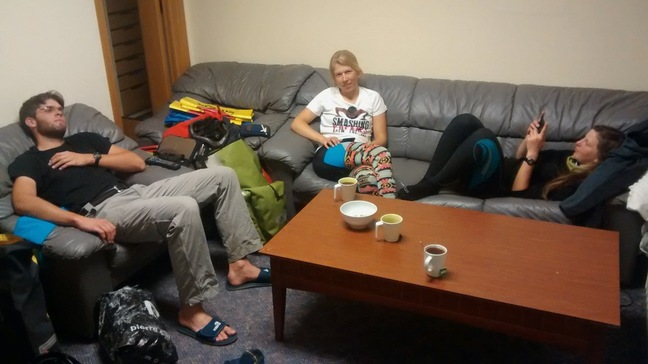
\includegraphics[width=.9\linewidth]{./photos/x-s-2014-08-17_23-52-35__112.jpg}
	\caption*{Wieczór. Nocleg. Ciepło i miękko.}
	\label{img:exhaustion}
\end{figure}%

\vfill

\pagebreak